\documentclass{beamer}
\usepackage{amsmath}
\usepackage{rotating}
\usepackage{graphicx}
\usepackage{multimedia}
\usepackage{listings}

\useinnertheme[shadow=true]{rounded}
\useoutertheme{shadow}
\usecolortheme{orchid}
\usecolortheme{whale}

\mode<presentation>

\newcommand{\dif}{\, \mathrm{d}}
\newcommand{\diff}[2]{\frac{\mathrm{d}#1}{\mathrm{d}#2}}
\newcommand{\partdiff}[2]{\frac{\partial #1}{\partial #2}}
\newcommand{\ub}[1]{\underbar{$#1$}\,}

\title{TMA4280 - Introduction to supercomputing}
\subtitle{Poisson solvers}
\author{Arne Morten Kvarving}
\institute{NTNU and SINTEF ICT}
\date{February 2014}

\begin{document}

\maketitle
\begin{frame}\frametitle{The problem at hand}
  \begin{itemize}
    \item We want to solve
      \[
        \ub{A}\ub{x} = \ub{b},\quad \ub{u},\ub{g} \in \mathbb{R}^N, \ub{A} \in \mathbb{R}^{NxN}.
      \]
      where $\ub{A}$ is the system resulting from discretizing a Poisson problem using finite differences.
    \item We use the standard notation for matrices and vectors, i.e.
      \[
        \begin{bmatrix}
          a_{11} & a_{12} & \cdots & a_{1N} \\
          a_{21} & a_{22} & \cdots & a_{2N} \\
          \vdots & \ddots \\
          a_{N1} & \cdots & & a_{NN}
        \end{bmatrix}	\begin{bmatrix}
          x_1 \\
          x_2 \\
          \ddots \\
          x_N
        \end{bmatrix} = \begin{bmatrix}
          b_1\\
          b_2 \\
          \ddots\\
          b_N
        \end{bmatrix}
      \]
  \end{itemize}
\end{frame}

\begin{frame}\frametitle{Computer algorithms}
  \begin{itemize}
    \item We know that the solution is given by
      \[
        \ub{x} = \ub{A}^{-1}\ub{b}.
      \]
    \item Explicitly forming the inverse $\ub{A}^{-1}$ is expensive, round-off prone
        and something we seldom do on computers.
    \item Rather we implement algorithms which solve a linear system given a 
        right-hand side vector.
    \item Which algorithm we (can) use is dependent on the structure and properties of
        the matrix $\ub{A}$.
  \end{itemize}
\end{frame}
\begin{frame}\frametitle{Computer algorithms}
  \begin{itemize}
    \item Trivial example: If $\ub{A}$ is orthogonal, then
      \[
        \ub{x} = \ub{A}^T\ub{b}.
      \]
    \item Orthogonal matrices are more the exception than a rule.
    \item We are more likely to exploit
      \begin{itemize}
        \item Symmetry
        \item Definiteness
        \item Sparsity
      \end{itemize}
    \item We will now consider different algorithms, their implementation and their
      usability in a parallel context.
  \end{itemize}
\end{frame}
\begin{frame}\frametitle{General matrices - the hammer of linear algebra}
  \begin{itemize}
    \item In your elementary course in linear algebra you learned two ways to invert
      general matrices.
      \item First was Cramer's rule: The solution to a linear system
        \[
          \ub{A}\ub{x} = \ub{b}
        \]
        can be found by repeatedly applying the rule
        \[
          x_i = \frac{\det\left(\ub{A}_i\right)}{\det\left(\ub{A}\right)}\quad \forall i
        \]
        where $\ub{A}_i$ is formed by replacing column $i$ in $\ub{A}$ with $\ub{b}$.
      \item Naive\footnote{Somebody found a smarter way in later years which does it in polynomial time}
            implementations scales as $N!$ - unusable in real-life calculations.
    \end{itemize}
\end{frame}
\begin{frame}\frametitle{General matrices - the hammer of linear algebra}
  \begin{itemize}
    \item Thus, we rather resort to Gaussian elimination. 
    \item This is a systematic procedure
      that allows us to transform the matrix $\ub{A}$ into a triangular form,
      which allows for easy inversion using backward substitutions.
      \[
        \begin{bmatrix}
          x & x & x & x & x \\
          0 & x & x & x & x \\ 
          0 & 0 & x & x & x \\ 
          0 & 0 & 0 & x & x \\ 
          0 & 0 & 0 & 0 & x
        \end{bmatrix}
      \]
    \item Last equation is trivial, solve that, plug value into next-to-last equation, which
      makes that trivial, rinse and repeat.
  \end{itemize}
\end{frame}
\begin{frame}\frametitle{General matrices - the hammer of linear algebra}
  \begin{itemize}
    \item The equations are on the form
      \[
        \begin{aligned}
          a_{11}x_1 &+ a_{12}x_2 &+ \cdots & +a_{1N}x_N &= b_1 \\
                                             a_{21}x_1 &+ a_{22}x_2 &+ \cdots & +a_{2N}x_N &= b_2 \\
                                                                                          &\ \vdots  & & &=\ \ \vdots
        \end{aligned}
      \]
    \item We want to get rid of the term $a_{21}x_1$. We do this by applying the
      row-operation $\left(\text{row 2}\right)-\frac{a_{21}}{a_{11}}\left(\text{row 1}\right)$.
    \item This yields
      \[
        \begin{aligned}
          a_{11}x_1 &+ a_{12}x_2 &+ \cdots & +a_{1N}x_N &= b_1 \\
                                                     0 &+ \left(a_{22}-\frac{a_{21}}{a_{11}}a_{12}\right)x_2 &+ \cdots & +a_{2N}x_N &= b_2 -\frac{a_{21}}{a_{11}}b_1 \\
                                                                                          &\ \vdots  & & &=\ \  \vdots
        \end{aligned}
      \]
  \end{itemize}
\end{frame}
\begin{frame}\frametitle{General matrices - the hammer of linear algebra}
  \begin{itemize}
    \item We now repeat this for all
      \begin{itemize}
        \item All rows,
        \item all columns beneath the diagonal.
      \end{itemize}
    \item Requirement: We need $a_{kk} \neq 0$. If not, we have to exchange two
      rows. This is called \emph{pivoting}.
    \item Additionally, since we are working in limited precision numbers, we want
      $a_{kk} \gg 0$ to limit cancellation errors. Thus, we should always choose
      the row with the largest $a_{kk}$ - this is called partial pivoting.
    \item This is a procedure with very simple rules $\Rightarrow$ very suitable for
      implementation on a computer.
  \end{itemize}
\end{frame}
\begin{frame}\frametitle{General matrices - the hammer of linear algebra}
  \begin{itemize}
    \item Two problems with vanilla Gaussian elimination:
      \begin{itemize}
        \item We also have to modify the right-hand side vector $\ub{b}$. This means
          that we have to redo the entire factorization if the vector changes.
        \item Even with partial pivoting, it is still rather prone to round-off errors.
      \end{itemize}
    \item For this reason, Gaussian elimination is usually implemented a bit differently
      on a computer. Rather than transforming the matrix $\ub{A}$ into triangular form,
      we seek two matrices $\ub{L}, \ub{U}$ such that $\ub{A} = \ub{L}\ub{U}$, where
      $\ub{L}$ is lower triangular and $\ub{U}$ is upper triangular.
    \item The factorization phase do not involve the vector $\ub{b}$ $\Rightarrow$
      it is reusable for different right-hand side vectors.
  \end{itemize}
\end{frame}
\begin{frame}\frametitle{General matrices - the hammer of linear algebra}
  \begin{itemize}
    \item We can then find the solution to a system through
      \[
        \begin{split}
                \ub{A}\ub{x} &= \ub{b} \\
          \ub{L}\ub{U}\ub{x} &= \ub{b} \Rightarrow \\
                \ub{L}\ub{v} &= \ub{b} \\
              \ub{U}{\ub{x}} &= \ub{v},
        \end{split}
      \]
      i.e. we first apply forward substitutions and the backward substitutions.
  \end{itemize}
\end{frame}
\begin{frame}\frametitle{General matrices - the hammer of linear algebra}
  \begin{itemize}
    \item There is a redundancy in this approach - we have two sets of diagonal values
      (one in $\ub{L}$, one in $\ub{U}$). This give rise to two alternative algorithms,
      Doolittle's method and Crout's method.
    \item We here consider Doolittle's method which chooses 1's on the diagonal of $\ub{L}$.
    \item The algorithm can be stated as
      \[
        \begin{aligned}
          u_{1k} &= a_{1k}\quad\ &k=1,\cdots,N \\
          l_{j1} &= \frac{a_{j1}}{u_{11}}\quad &j=2,\cdots,N \\
          u_{jk} &= a_{jk}-\sum_{s=1}^{j-1}l_{js}u_{sk}\quad &k=j,\cdots,N, j \geq 2 \\
          l_{jk} &= \frac{1}{u_{kk}}\left(a_{jk}-\sum_{s=1}^{k-1}l_{js}u_{sk}\right)\quad &j=k+1,\cdots,N, k \geq 2.
        \end{aligned}
      \]
  \end{itemize}
\end{frame}
\begin{frame}\frametitle{LAPACK}
  \begin{itemize}
    \item LU factorization is somewhat tedious to implement, in particular in an efficient way.
    \item Smart people have done this for you.
    \item \emph{LAPACK} - The Linear Algebra PACK builds on the \emph{BLAS}.
    \item Same naming conventions and matrix formats.
    \item Just like with BLAS and CBLAS, there is a LAPACK and CLAPACK.
    \item We stick to LAPACK (Fortran conventions).
  \end{itemize}
\end{frame}
\begin{frame}\frametitle{LAPACK}
  \begin{itemize}
    \item Function prototype:
      \lstinputlisting[basicstyle=\small]{prototype.c}
    \item Usage:
      \lstinputlisting[basicstyle=\small]{solve-lu.c}
  \end{itemize}
\end{frame}
\begin{frame}\frametitle{LAPACK}
  \begin{itemize}
    \item \emph{dgesv} overwrites the matrix $\ub{A}$ with the factorization $\ub{L}, \ub{U}$.
    \item \emph{dgesv} is actually calling two functions;
      \begin{itemize}
        \item First it calls \emph{dgetrf} to factorize the matrix.
        \item Then it calls \emph{dgetrs} to solve the system.
      \end{itemize}
    \item Thus, after the first call, if we store the pivot numbers we can solve
      for different right-hand sides (see common library code).
  \end{itemize}
\end{frame}
\begin{frame}\frametitle{Improving the performance}
  \begin{itemize}
    \item While \emph{LAPACK} is efficiently implemented, it cannot do wonders.
    \item LU-factorization scales as $\mathcal{O}\left(N^3\right)$.
    \item Totally unrealistic numbers, but just to give you an idea of how this scales:
      \begin{figure}
        \begin{tabular}{c|c}
          $N$ & $T$ \\
          \hline
          $10$ & 1000s = 17min \\
         $100$ & $1\cdot 10^6$s = 11 days \\
         $1000$ & $1\cdot 10^9$s = 31 years 
        \end{tabular}
       \end{figure}
     \item Even if $\ub{A}$ is sparse, $\ub{L}$ and $\ub{U}$ is in general not.
     \item Typically you get fill in $2b$ diagonals, where $b$ is the bandwidth
       of the (renumbered) matrix $\ub{A}$.
     \item We can do slightly better by exploiting symmetry.
  \end{itemize}
\end{frame}
\begin{frame}\frametitle{Improving the performance}
  \begin{itemize}
    \item If $\ub{A}$ is symmetric and positive definite, we find that $\ub{U}=\ub{L}^T$.
    \item Thus we can save a factor 2 in memory and a factor 2 in required FLOP.
    \item Furthermore, no pivoting is required for such systems.
    \item This is called Cholesky factorization.
  \end{itemize}
\end{frame}
\begin{frame}\frametitle{Cholesky factorization}
  \begin{itemize}
    \item Function prototype:
      \lstinputlisting[basicstyle=\small]{chol.c}
    \item Usage:
      \lstinputlisting[basicstyle=\small]{solve-chol.c}
  \end{itemize}
\end{frame}
\begin{frame}\frametitle{Improving the performance}
  \begin{itemize}
     \item LU-factorization is very unfit for parallel implementations.
       \begin{itemize}
         \item It is sequential in nature (you need to eliminate for row 2 before you
           can start to eliminate for row 3).
         \item Pivoting requires syncronization for every row.
         \item Substitution phase is completely sequential (less important).
         \item There have been some smart people working on this, looking at the
           graph of the matrix to identify independent blocks.
       \end{itemize}
     \item For most systems, the results are mediocre and only scale to a 
           few processes/threads.
     \item Simply put, LU factorization is unusable as a solver in a parallel context.
     \item However, it is very often utilized as a component in other algorithms.
  \end{itemize}
\end{frame}
\begin{frame}\frametitle{Better approaches}
  \begin{itemize}
    \item Solution methods can be categorized in two classes: 
      \begin{itemize}
        \item Direct methods - these are methods which yields the solution in
          a countable number of operations - LU factorization is a prime example of this.
        \item Iterative methods, which find the solution through applying some
          iterative procedure. Not as easy to exactly count the required number
          of operations.
      \end{itemize}
    \item We now consider another example of a direct method.
  \end{itemize}
\end{frame}
\begin{frame}\frametitle{Diagonalization}
  \begin{itemize}
    \item This is not a hammer. We need to exploit properties of the linear system at hand.
    \item We recall the five-point formula;
      \begin{figure}[H]
        \begin{center}
          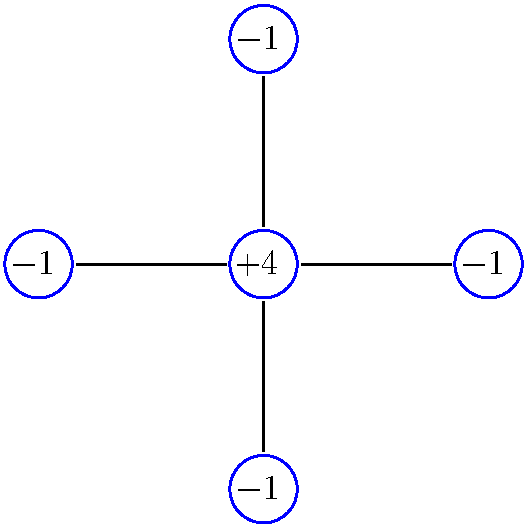
\includegraphics[width=3cm]{../../notes/07.poisson-fdm/FivePointStencil}
        \end{center}
      \end{figure}
    \item This results from using the three-point formula in each spatial direction;
      \begin{figure}[H]
        \begin{center}
          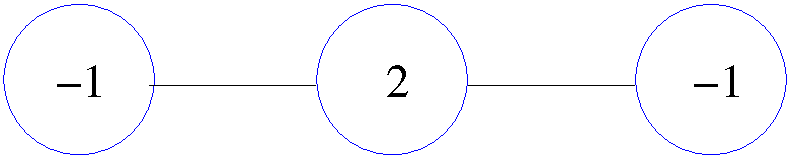
\includegraphics[width=3cm]{../../notes/07.poisson-fdm/ThreePointStencil}
        \end{center}
      \end{figure}
  \end{itemize}
\end{frame}
\begin{frame}\frametitle{Diagonalization contd.}
  \begin{itemize}
    \item In the following, we refer to the matrix resulting from applying the five-point formula
      as $\ub{A}$, while the matrix we obtain from applying the three-point formula to
      a 1D problem, we refer to as $\ub{T}$.
    \item For any SPD matrix $\ub{C}$, we know that we can perform an eigendecomposition;
      \[
        \ub{C}\ub{Q} = \ub{Q}\ub{\Lambda},
      \]
      where $\ub{Q}$ is the matrix with the eigenvectors of $\ub{C}$ as columns,
      and $\ub{\Lambda}$ is a diagonal matrix with the corresponding eigenvalues on
      the diagonal.
    \item Since $\ub{Q}$ is an orthogonal matrix, we equivalently have
      \[
        \ub{C} = \ub{Q}\ub{\Lambda}\ub{Q}^T.
      \]
  \end{itemize}
\end{frame}
\begin{frame}\frametitle{Diagonalization contd.}
  \begin{itemize}
    \item We plug this into a linear system of equations, i.e.
      \[
        \begin{split}
          \ub{C}\ub{x} &= \ub{b} \Rightarrow \\
          \ub{Q}\ub{\Lambda}\ub{Q}^T\ub{x} &= \ub{b}.
        \end{split}
      \]
    \item We multiply with $\ub{Q}^T$ from the left,
          recalling at $\ub{Q}^T = \ub{Q}^{-1}$;
      \[
        \ub{\Lambda}\underbrace{\ub{Q}^T\ub{x}}_{\tilde{\ub{x}}} = \underbrace{\ub{Q}^T\ub{f}}_{\ub{\tilde{b}}}
      \]
    \item Thus, we can now solve the system in three steps.
  \end{itemize}
\end{frame}
\begin{frame}\frametitle{Diagonalization contd.}
  \begin{enumerate}
    \item We calculate $\ub{b}$ through a matrix-vector product.
      \[
        \ub{\tilde{b}} = \ub{Q}^T\ub{x}
      \]
      in $\mathcal{O}\left(N^2\right)$ operations.
    \item We solve the system
      \[
        \ub{\Lambda}\ub{\tilde{x}} = \ub{\tilde{b}}
      \]
      in $\mathcal{O}\left(N\right)$ operations (remember - $\ub{\Lambda}$ is diagonal).
    \item We finally find the solution to the system through another matrix-vector product;
      \[
        \ub{x} = \ub{Q}\ub{\tilde{x}}
      \]
      in $\mathcal{O}\left(N^2\right)$ operations.
  \end{enumerate}
\end{frame}
\begin{frame}\frametitle{Diagonalization contd.}
  \begin{itemize}
    \item This looks promising - it seems we just found a way to solve the system in
      $\mathcal{O}\left(N^2\right)$ operations instead of $\mathcal{O}\left(N^3\right)$!
    \item Sadly not true - as we have to find the eigen decomposition of the matrix.
    \item This scales as $\mathcal{O}\left(N^3\right)$ so we are back to square 1.
    \item However, if we consider a certain 2D problems, this changes.
  \end{itemize}
\end{frame}
\begin{frame}\frametitle{Diagonalization contd.}
  \begin{itemize}
    \item We constructed the $\ub{A}$ matrix as the sum of applying the three-point
      formula in $x$ and $y$.
    \item In the language of linear algebra, this translates to a tensor-product, that is
      \[
        \ub{A} = \ub{I}\otimes\ub{T} + \ub{T}\otimes\ub{I}.
      \]
    \item It turns out we have a very nice relation we can use here.
    \item If we have an operator on this form in a global numbering scheme, and
      an associated linear system
      \[
        \ub{A}\ub{x} = \ub{b}
      \]
      we can equivalently state this is
      \[
        \ub{T}\ub{X} + \ub{X}\ub{T}^T = \ub{B}
      \]
      in a local numbering scheme.
  \end{itemize}
\end{frame}
\begin{frame}\frametitle{Diagonalization contd.}
  \begin{itemize}
    \item A global numbering scheme is a scheme where we number the unknowns using a single index
      - this naturally maps to a vector.
    \item A local numbering scheme is a scheme where we number the unknowns using one index for each spatial direction
      - this naturally maps to a matrix.
    \item Thus, we consider a system of matrix equations.
    \item An alternative way of deriving the equations; we first operate with $\ub{T}$
      along the columns of $\ub{X}$, then along the rows of $\ub{X}$, i.e.
      \[
        \underbrace{\ub{T}\ub{X}}_{\text{operate along columns, i.e. in x}} + \underbrace{\left(\ub{T}\ub{X}^T\right)^T}_{\text{operate along rows, i.e. in y}}.
      \]
  \end{itemize}
\end{frame}
\begin{frame}\frametitle{Diagonalization contd.}
  \begin{itemize}
    \item We now plug the diagonalization of $\ub{T}$ into the discretization
      of the 2D Poisson problem, recalling that $\ub{T}$ is symmetric;
      \[
        \begin{split}
          \ub{T}\ub{X} + \ub{X}\ub{T} &= \ub{B} \Rightarrow \\
          \ub{Q}\ub{\Lambda}\ub{Q}^T\ub{X} + \ub{X}\ub{Q}\ub{\Lambda}\ub{Q}^T &= \ub{B}.
        \end{split}
      \]
    \item We multiply with $\ub{Q}$ from the right
      \[
        \ub{Q}\ub{\Lambda}\ub{Q}^T\ub{X}\ub{Q} + \ub{X}\ub{Q}\ub{\Lambda} = \ub{B}\ub{Q}.
      \]
    \item We then multiply with $\ub{Q}^T$ from the left;
      \[
        \ub{\Lambda}\underbrace{\ub{Q}^T\ub{X}\ub{Q}}_{\ub{\tilde{X}}} + \underbrace{\ub{Q}^T\ub{X}\ub{Q}}_{\ub{\tilde{X}}}\ub{\Lambda} = \underbrace{\ub{Q}^T\ub{B}\ub{Q}}_{\ub{\tilde{B}}},
      \]
      or
      \[
        \ub{\Lambda}\ub{\tilde{X}} + \ub{\tilde{X}}\ub{\Lambda} = \ub{\tilde{B}}.
      \]
  \end{itemize}
\end{frame}
\begin{frame}\frametitle{Diagonalization contd.}
  We then find the solution in three steps
  \begin{enumerate}
    \item We calculate $\ub{\tilde{B}}$ through two matrix-matrix products.
      \[
        \ub{\tilde{B}} = \ub{Q}^T\ub{B}\ub{Q}.
      \]
      in $\mathcal{O}\left(N^3\right)$ operations.
    \item We solve the system
      \[
        \begin{split}
          \tilde{x}_{ij} = \frac{\tilde{b}_{ij}}{\lambda_i+\lambda_j}\quad 1 \leq i,j \leq N
        \end{split}
      \]
      in $\mathcal{O}\left(N^2\right)$.
    \item We finally find the solution to the system through two matrix-matrix products;
      \[
        \ub{X} = \ub{Q}\ub{\tilde{X}}\ub{Q}^T
      \]
      in $\mathcal{O}\left(N^3\right)$ operations.
  \end{enumerate}
\end{frame}
\begin{frame}\frametitle{Diagonalization contd.}
  \begin{itemize}
    \item We now have a very fast algorithm.
    \item The operation count scales very well with the number of unknowns - just $\mathcal{O}\left(N\right)$ work per unknown.
    \item It scales perfectly in memory - we just need $\mathcal{O}\left(N^2\right)$ datas (a few numbers per unknown).
    \item It is also parallelizable - a few large, global data exchanges would be needed
      (the transpositions of the matrix). You will get to study how this scales in exercise 6.
    \item Compare this to LU factorization - which would required
      $\mathcal{O}\left(M^2\right) = \mathcal{O}\left((N^2)^6\right) = \mathcal{O}\left(N^6\right)$ operations
      and
      $\mathcal{O}\left(N^4\right)$ storage.
    \item It beats sparse/banded LU as well. It would require
      $\mathcal{O}\left(N^4\right)$ operations and $\mathcal{O}\left(N^3\right)$ storage.
  \end{itemize}
\end{frame}
\begin{frame}\frametitle{Diagonalization contd.}
  \begin{itemize}
    \item The diagonalization method is quite general, applicable to any SPD system with
      a tensor-product operator.
    \item We used the particular problem to make it more easily understandable (I hope!)
    \item It turns out that if we use more information from the Poisson problem,
      we can do even better!
  \end{itemize}
\end{frame}
\begin{frame}\frametitle{Diagonalization contd.}
  \begin{itemize}
    \item The continuous eigenvalue problem
      \[
        \begin{split}
              -u_{xx} &= \lambda u \quad \text{in } \Omega=(0,1)\\
          u(0) = u(1) &= 0.
        \end{split}
      \]
      has solutions
      \[
         \begin{split}
            \bar{u}_j(x) &= \sin(j \pi x), \\
            \bar{\lambda}_j &= j^2 \pi^2,
         \end{split}
         \qquad j=1,2,\ldots,\infty.
      \]
    \item We now consider operating with $\ub{T}$ on vectors consisting of $\bar{u}_j$
      sampled in the grid points $x_i, i=1,\ldots,N-1$, i.e.
      \[
        \left(\bar{q}_j\right)_i = \bar{u}_j\left(x_i\right) = \sin\left(\frac{ij\pi}{N}\right).
      \]
  \end{itemize}
\end{frame}
\begin{frame}\frametitle{Diagonalization contd.}
  \begin{itemize}
    \item This yields
      \[
        \left(\ub{T}\ub{\bar{q}}_j\right)_i = \underbrace{2\left(1-\cos\left(\frac{j\pi}{N}\right)\right)}_{\lambda j}\underbrace{\sin\left(\frac{ij\pi}{N}\right)}_{\left(\bar{q}_j\right)_i}.
      \]
     \item Thus, if we normalize these vectors, we have found the eigenvalues and eigenvectors of $\ub{T}$!
     \item Normalization: $\ub{q}_j = \alpha\ub{\bar{q}}_j$ s.t.
       \[
         \begin{split}
           \ub{q}_j^T\ub{q}_j = 1 \Rightarrow
           \left(\ub{q}_j\right)_i &= \sqrt{\frac{2}{N}}\sin\left(\frac{ij\pi}{N}\right). \\ 
                         \lambda_j &= 2\left(1-\cos\left(\frac{j\pi}{N}\right)\right).
         \end{split}
       \]
  \end{itemize}
\end{frame}
\begin{frame}\frametitle{The discrete Fourier transform}
  \begin{itemize}
    \item We consider a periodic function $v(x)$ with period $2\pi$.
    \item We sample this function at equidistant points $x_j, j=0,1, \ldots, N, x_j = jh, h=\frac{2\pi}{N}$.
    \item We name the samples $v_j = v\left(x_j\right)$.
      \begin{figure}[H]
        \centering
        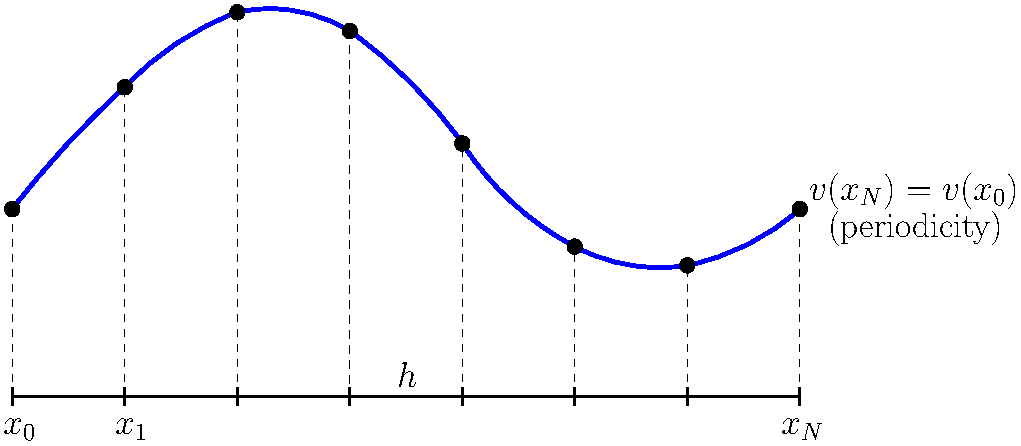
\includegraphics[width=7cm]{../../notes/08.poisson-diag/PeriodicFunction}
      \end{figure}
  \end{itemize}
\end{frame}
\begin{frame}\frametitle{The discrete Fourier transform contd.}
  \begin{itemize}
    \item Consider the vectors $\ub{\varphi}_k$, where
      \[
        \left(\ub{\varphi}_k\right)_j = e^{ikx_j},
      \]
      where
      \[
        e^{ikx_j} = \cos\left(kx_j\right)+i\sin\left(kx_j\right).
      \]
    \item These vectors form a basis for the $N$-dimensional space $\mathbb{C}^N$.
        In particular
        \[
          \underline{\varphi}_k^H \underline{\varphi}_l = 
          \begin{cases}
            N, & k=l, \\
            0, & k \not= l,
          \end{cases}
          \qquad \qquad k,l=0,1,\ldots,N-1.
        \]
  \end{itemize}
\end{frame}
\begin{frame}\frametitle{The discrete Fourier transform contd.}
  \begin{itemize}
    \item Since these form a basis, any vector in the space can be expressed
      as a linear combination of these vectors.
    \item The vector 
      \begin{equation*}
        \underline{v} = 
        \begin{bmatrix}
          v_0 \\
          \vdots \\
          v_{N-1}
        \end{bmatrix}
        \in \mathbb{R}^N
      \end{equation*}
      can be expressed in this basis as

      \begin{align*}
        \underline{v} &= \sum_{k=0}^{N-1} \hat{v}_k \underline{\varphi}_k \\
        \intertext{or}
        v_j &= \sum_{k=0}^{N-1} \hat{v}_k (\underline{\varphi}_k)_j = \sum_{k=0}^{N-1} \hat{v}_k e^{ik x_j}.
      \end{align*}
  \end{itemize}
\end{frame}
\begin{frame}\frametitle{The discrete Fourier transform contd.}
  \begin{itemize}
    \item Here $\hat{v}_k$, are the discrete Fourier coefficients given by
      \begin{equation*}
        \hat{v}_k = \frac{1}{N} \sum_{j=0}^{N-1} v_j e^{-ik x_j}, \qquad \qquad 
        \begin{matrix}
          x_j = j h \\
          h = \frac{2\pi}{N}
        \end{matrix}
        \qquad k=0,1,\ldots,N-1
      \end{equation*}
    \item The Fourier transform is extremely useful and has been extensively studied.
    \item Example where it is used: Signal analysis, audio compression, video compression.
    \item Important in the following: The DFT coefficients of an odd signal are imaginary.
  \end{itemize}
\end{frame}
\begin{frame}\frametitle{The discrete Sine transform}
  \begin{itemize}
    \item A related transformation is the discrete sine transform, \emph{DST}.
    \item It is applicable to a function $v(x)$ which is periodic with period
        $2\pi$ and \emph{odd}, i.e. $v(x) = -v(x+\pi)$.
     \item We discretize this function on a equidistant mesh between $0$ and $\pi$.
     \item Since $v$ is odd, we know that $v\left(x_0\right) = v\left(x_N\right) = 0$.
     \item Thus the discrete function is represented by the vector
       \[
        \underline{v} = 
        \begin{bmatrix}
          v_1 \\
          \vdots \\
          v_{n-1}
        \end{bmatrix}
        \in \mathbb{R}^{n-1}.
      \]
  \end{itemize}
\end{frame}
\begin{frame}\frametitle{The discrete Sine transform}
  \begin{itemize}
    \item A basis for this space of (discrete) functions is given by
    \begin{align*}
      (\underline{\psi}_k)_j &= \sin \biggl( \frac{k j \pi}{n} \biggr), \qquad j=1,\ldots,n-1, \\
      \intertext{and with}
      \underline{\psi}_k^T \underline{\psi}_l &=
      \begin{cases}
        \frac{n}{2}, & k=l, \\
        0, & k \not= 0.
      \end{cases}
    \end{align*}
    \item Thus
      \begin{alignat*}{2}
        v_j &= \sum_{k=1}^{n-1} \widetilde{v}_k \sin \biggl( \frac{k j \pi}{n} \biggr) = \ub{S}^{-1}\tilde{\ub{v}}, &\qquad j&=1,\ldots,n-1, \\
        \intertext{where}
        \widetilde{v}_k &= \frac{2}{n} \sum_{j=1}^{n-1} v_j \sin \biggl( \frac{j k \pi}{n} \biggr)=\ub{S}\ub{v}, &\qquad  k&=1,\ldots,n-1.
      \end{alignat*}
  \end{itemize}
\end{frame}
\begin{frame}\frametitle{The DFT and DST relationship}
  \begin{itemize}
    \item In particular we have that
      \[
        \ub{Q} = \sqrt{\frac{N}{2}}\ub{S}, \ub{Q}^T = \sqrt{\frac{2}{N}}\ub{S}^{-1}.
      \]
    \item Consider a vector
      \begin{align*}
        \underline{v} &= 
        \begin{bmatrix}
          v_1 \\
          \vdots \\
          v_{n-1}
        \end{bmatrix}
        \in \mathbb{R}^{n-1}. \\
        \intertext{\small Construct the extended vector as an ``odd'' extension}
        w &=
        \begin{bmatrix}
          0 \\ 
          v_1 \\
          \vdots \\
          v_{n-1} \\
          0 \\
          -v_{n-1} \\
          \vdots \\
          -v_1
        \end{bmatrix}
        \in \mathbb{R}^{2n}.
      \end{align*}
      \normalsize
  \end{itemize}
\end{frame}
\begin{frame}\frametitle{The DFT and DST relationship contd.}
  \begin{itemize}
    \item It turns out that the DST coefficients of $\ub{v}$ and the DFT coefficients
      of $\ub{w}$ are related through
      \[
        \tilde{v}_k = 2i\tilde{w}_k, k = 1,\ldots,N-1.
      \]
    \item Thus we can find the DST of a vector by taking the DFT of the odd extension,
      then multiplying the first $N-1$ coefficients with $2i$ and throwing away the rest.
    \item There exists fast methods for computing the DFT of a signal, in particular the
      infamous \emph{Fast Fourier Transform} method.
    \item Requires\footnote{There are generalizations which do not} $N$ to be a power-of-two.
    \item This manages to find the coefficients in $\mathcal{O}\left(N^2\log N\right)$ for $N^2$ coefficients.
    \item Faster than calculating them through matrix-vector products since this is $\mathcal{O}\left(N^3\right)$.
  \end{itemize}
\end{frame}
\begin{frame}\frametitle{Diagonalization using DST}
  We then find the solution in three steps
  \begin{enumerate}
    \item We calculate $\ub{\tilde{B}}$ through
      \[
        \ub{\tilde{B}}^T = \ub{S}^{-1}\left(\left(\ub{S}\ub{B}\right)^T\right)
      \]
      in $\mathcal{O}\left(N^2\log N\right)$ operations.
    \item We solve the system
      \[
        \begin{split}
          \tilde{x}_{ij} = \frac{\tilde{b}_{ij}}{\lambda_i+\lambda_j}\quad 1 \leq i,j \leq N
        \end{split}
      \]
      in $\mathcal{O}\left(N^2\right)$.
    \item We finally find the solution to the system through 
      \[
        \ub{X} = \ub{S}^{-1}\left(\ub{S}\left(\ub{\tilde{X}}^T\right)\right)^T
      \]
      in $\mathcal{O}\left(N^2\log N\right)$ operations.
  \end{enumerate}
\end{frame}
\begin{frame}\frametitle{Iterative methods}
  \begin{itemize}
    \item This far we have considered direct methods which work on the matrix itself.
    \item Now: iterative methods.
    \item Iterative methods seek to solve the system by iterations, gradually improving an estimate of
      the solution.
    \item In general they do not yield the exact solution, but rather an approximation.
    \item A very important concept in iterative methods: The residual:
      \[
        \ub{r} = \ub{b}-\ub{A}\ub{x}^k
      \]
      for some iteration level $k$.
    \item Obviously $\ub{r}$ is 0 for the exact solution $\ub{x}$.
    \item Used to measure how far we are from the actual solution to the system.
  \end{itemize}
\end{frame}
\begin{frame}
\frametitle{Fixed point iterations}
\begin{itemize}
  \item Tempting to try the iterative schemes we learned in elementary calculus.
  \item Fixed point iterations require us to write the problem on the from $\ub{x} = g(\ub{x})$ for some function $g$;
    \[
      \begin{split}
        \ub{f}(\ub{x}) &= \ub{0} = \ub{g}(\ub{x})-\ub{x} \\
        \ub{A}\ub{x}-\ub{b} &= \ub{0} = \ub{g}(\ub{x})-\ub{x} \Rightarrow \\
        (\ub{A}+\ub{I})\ub{x}-\ub{b} = \ub{x} \Rightarrow
        \ub{x}^{k+1} &= (\ub{A}+\ub{I})\ub{x}^k-\ub{b}
      \end{split}
    \]
    This will work in extremely few since the requirement that $\ub{g}$ is a contraction
    is requiring that
    \[
      \max_{i}|\lambda_i(\ub{I}+\ub{A})| < 1
    \]
    which is seldom the case.
  \end{itemize}
\end{frame}
\begin{frame}
\frametitle{Newton iterations}
  \begin{itemize}
    \item Newton iterations works on a system on the form $F(\ub{x}) = \ub{0}$:
      \[
        \ub{x}^{k+1} = \ub{x}^k-\ub{A}^{-1}\left(\ub{A}\ub{x}^k-\ub{b}\right) = \ub{A}^{-1}\ub{b}.
      \]
      Doh! That is the problem we want to solve in the first place :(
  \end{itemize}
\end{frame}
\begin{frame}\frametitle{Splitting based iterative methods.}
  \begin{itemize}
    \item Again we consider a linear system
      \[
        \ub{A}\ub{x} = \ub{b}.
      \]
    \item We split the matrix $\ub{A}$ in three parts; \tiny
      \[
        \begin{split}
          \ub{A} &= \ub{L} + \ub{D} + \ub{U} \\
                 &= \begin{bmatrix}
                      0 & \\
                      a_{21} & 0\\
                      a_{31} & a_{32} & 0\\
                      \ddots & \ddots & \ddots & \ddots
                    \end{bmatrix} +
                    \begin{bmatrix}
                      a_{11} \\
                             & a_{22} \\
                             &        & a_{33} \\
                             &        &       & \ddots
                    \end{bmatrix}+
                    \begin{bmatrix}
                      0 & a_{12} & \dots \\
                      0 & 0      & a_{23} & \dots \\
                      0 & 0      & 0      & a_{34}  \\
                      0 & 0      & 0      & 0 & \ddots
                    \end{bmatrix}
        \end{split}
      \] \normalsize
    \item Do \emph{NOT} confuse these $\ub{L}$ and $\ub{U}$ matrices with the $\ub{L}\ub{U}$ factorization (Gaussian elimination).
  \end{itemize}
\end{frame}
\begin{frame}\frametitle{Splitting based iterative methods contd.}
  \begin{itemize}
    \item Again we consider a linear system
      \[
        \ub{A}\ub{x} = \left(\ub{L}+\ub{D}+\ub{U}\right)\ub{x} = \ub{b}.
      \]
    \item This is the departure point for two well known iterative schemes. First: Gauss-Jacobi.
    \item We reorganize the system as
      \[
        \ub{D}\ub{x} = \ub{b}-\left(\ub{L}+\ub{U}\right)\ub{x}.
      \]
    \item We then make this into an iterative scheme by defining iteration level $k$:
      \[
        \ub{D}\ub{x}^{k+1} = \ub{b}-\left(\ub{L}+\ub{U}\right)\ub{x}^{k}.
      \]
  \end{itemize}
\end{frame}
\begin{frame}\frametitle{Splitting based iterative methods contd.}
  \begin{itemize}
    \item Likewise, we have the Gauss-Seidel scheme.
    \item We reorganize the system as
      \[
        \left(\ub{L}+\ub{D}\right)\ub{x} = \ub{b}-\ub{U}\ub{x}.
      \]
    \item We then make this into an iterative scheme by defining iteration level $k$:
      \[
        \left(\ub{L}+\ub{D}\right)\ub{x}^{k+1} = \ub{b}-\ub{U}\ub{x}^{k}.
      \]
    \item Can you tell the principal difference between these two methods?
  \end{itemize}
\end{frame}
\begin{frame}\frametitle{Splitting based iterative methods contd.}
  \begin{itemize}
    \item It is easy to spot on component form.
    \item Gauss-Jacobi:
      \[
        a_{ii}x_i^{k+1} = b_i - \sum_{j=1, j\neq i}^{N} a_{ij}x_j^k, \quad i=1,\dots,N.
      \]
    \item Gauss-Seidel:
      \[
        a_{ii}x_i^{k+1} = b_i - \sum_{j=1}^{i-1} a_{ij}x_j^{k+1} - \sum_{j=i+1}^Na_{ij}x_j^k, \quad i=1,\dots,N.
      \]
    \item Gauss-Seidel uses new iteration values as soon as they are available.
  \end{itemize}
\end{frame}
\begin{frame}\frametitle{Splitting based iterative methods contd.}
  \begin{itemize}
    \item These methods are very simple, and quite limited in their applicability.
    \item Gauss-Jacobi require that the spectral radius of $\ub{R} = \ub{D}^{-1}\left(\ub{L}+\ub{U}\right)$ is less than one, i.e.
      \[
        \rho(\ub{D}^{-1}\ub{R}) < 1.
      \]
    \item One way to guarantee that this is the case is if $\ub{A}$ is strictly diagonally dominant, i.e.
      \[
        |a_{ii}| > \sum_{j=1,j\neq i}^N |a_{ij}| \quad \forall i.
      \]
    \item This is \emph{NOT} the case for the Poisson operator. But it will still converge, although very slow.
    \item Gauss-Seidel is less strict, only requiring $\ub{A}$ to be SPD.
  \end{itemize}
\end{frame}
\begin{frame}\frametitle{Splitting based iterative methods contd.}
  \begin{itemize}
    \item A naive Gauss-Jacobi implementation might look like:
      \lstinputlisting[basicstyle=\tiny]{gj-naive.c}
  \end{itemize}
\end{frame}
\begin{frame}\frametitle{Splitting based iterative methods contd.}
  \begin{itemize}
    \item A naive Gauss-Jacobi with a residual tolerance might look like:
      \lstinputlisting[basicstyle=\tiny]{gj-naive-rtol.c}
  \end{itemize}
\end{frame}
\begin{frame}\frametitle{Splitting based iterative methods contd.}
  \begin{itemize}
    \item A naive Gauss-Seidel implementation might look like:
      \lstinputlisting[basicstyle=\tiny]{gs-naive.c}
  \end{itemize}
\end{frame}
\begin{frame}\frametitle{Splitting based iterative methods contd.}
  \begin{itemize}
    \item A naive Gauss-Seidel with a residual tolerance might look like:
      \lstinputlisting[basicstyle=\tiny]{gs-naive-rtol.c}
  \end{itemize}
\end{frame}
\begin{frame}\frametitle{Parallelizing Gauss-Jacobi iterations - threads}
  \begin{itemize}
    \item The Gauss-Jacobi iterations are easily parallelized.
    \item We simply fork the threads on the rows of the matrix.
      \lstinputlisting[basicstyle=\tiny]{gj-threads.c}
  \end{itemize}
\end{frame}
\begin{frame}\frametitle{Matrix-free iterations}
  \begin{itemize}
    \item The direct methods are characterized by the fact that we have to explicitly store
          the matrix (in a dense or sparse matrix).
    \item Iterative methods, however, do not care. As long as we obtain the value of the matrix-vector
          product, they do not care how we do it.
    \item This allows us to heavily optimize the Gauss-Jacobi iterations.
    \item We can avoid forming the matrix completely.
  \end{itemize}
\end{frame}
\begin{frame}\frametitle{Matrix-free Gauss-Jacobi iterations}
   \lstinputlisting[basicstyle=\tiny]{gj-threads-mfree.c}
\end{frame}
\begin{frame}\frametitle{Parallelizing Gauss-Seidel iterations - threads}
  \begin{itemize}
    \item The Gauss-Seidel iterations are more difficult to parallelize.
    \item This is due to the immediate data reuse, which implies a serial procedure.
    \item There is simply no way to implement the same algorithm in a parallel fashion.
    \item However, there is nothing that mandates that we sweep the unknowns in a particular order.
    \item If we change the order we sweep the unknowns, we can obtain a parallel algorithm.
  \end{itemize}
\end{frame}
\begin{frame}\frametitle{Parallelizing Gauss-Seidel iterations - threads}
  \begin{itemize}
    \item We color the nodes in a two-color alternating fashion.
       \begin{figure}[H]
        \begin{center}
          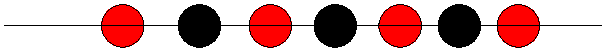
\includegraphics[width=9cm]{redblack}
        \end{center}
      \end{figure}
    \item Now, \textcolor{red}{red} nodes only couple to \textcolor{black}{black} nodes.
    \item We can thus sweep all \textcolor{red}{red} nodes in parallel, and then sweep all black nodes in parallel.
    \item Again: this \emph{changes} the algorithm; we cannot expect the same iteration history as in the serial implementation.
  \end{itemize}
\end{frame}
\begin{frame}\frametitle{Parallelizing Gauss-Seidel iterations - threads}
   \lstinputlisting[basicstyle=\tiny]{gs-threads-rb.c}
\end{frame}
\begin{frame}\frametitle{Iterative schemes - redundant storage}
  \begin{itemize}
    \item Another freedom offered by the iterative schemes is that we can store data as we see fit.
    \item For the direct methods, we eliminated the nodes on the boundary, since they are not
      part of the equation systems.
    \item We have no such restrictions for the iterative schemes, we are free to explicitly store the
      zeros on the boundaries.
    \item This is actually very beneficial, in particular when we consider MPI parallelization as we will see shortly.
  \end{itemize}
\end{frame}
\begin{frame}\frametitle{Gauss-Jacobi iterations with redundant storage}
   \lstinputlisting[basicstyle=\tiny]{gj-threads-mfree-redundant.c}
\end{frame}
\begin{frame}\frametitle{Gauss-Jacobi iterations - MPI parallelization}
  \begin{itemize}
    \item There are basically two ways to we can partition a linear system of equations
      \begin{enumerate}
        \item We can partition the data structure (the matrix and vector).
        \item We can partition the problem which generated the linear system in the first place - this is referred to as domain decomposition.
      \end{enumerate}
    \item The second approach is connected to the first approach.
          In particular, it can be seen as a particular way of splitting the data structure (more on this later).
  \end{itemize}
\end{frame}
\begin{frame}\frametitle{Matrix partitioning}
\begin{itemize}
  \item Row based division:
     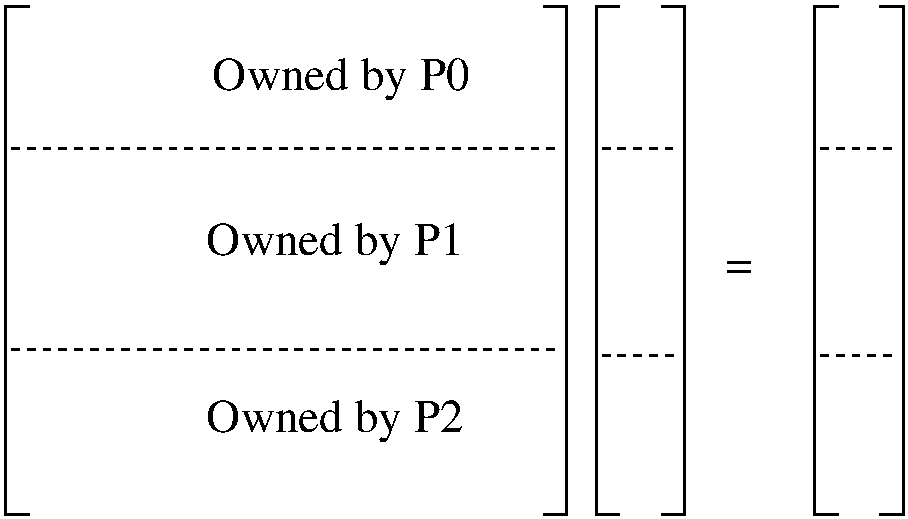
\includegraphics[width=7cm]{rows}
  \item Can be written on block form as
        \[
           \begin{bmatrix}
                \mathbf{A}_0 \\
                \mathbf{A}_1 \\
                \mathbf{A}_2
           \end{bmatrix}\begin{bmatrix}
                          \mathbf{x}_0 \\
                          \mathbf{x}_1 \\
                          \mathbf{x}_2
                        \end{bmatrix} = \begin{bmatrix}
                                          \mathbf{b}_0 \\
                                          \mathbf{b}_1 \\
                                          \mathbf{b}_2
                                        \end{bmatrix}
        \]
\end{itemize}
\end{frame}
\begin{frame}\frametitle{Matrix partitioning}
\begin{itemize}
  \item Thus we see that process $p$ can evaluate in two steps;
  \begin{enumerate}
    \item Collect entire vector $\mathbf{r}$.
    \item Perform local MxV $\mathbf{A}_p \mathbf{r}$.
  \end{enumerate}
\end{itemize}
\end{frame}
\begin{frame}\frametitle{Matrix partitioning}
\begin{itemize}
  \item Column based division:
     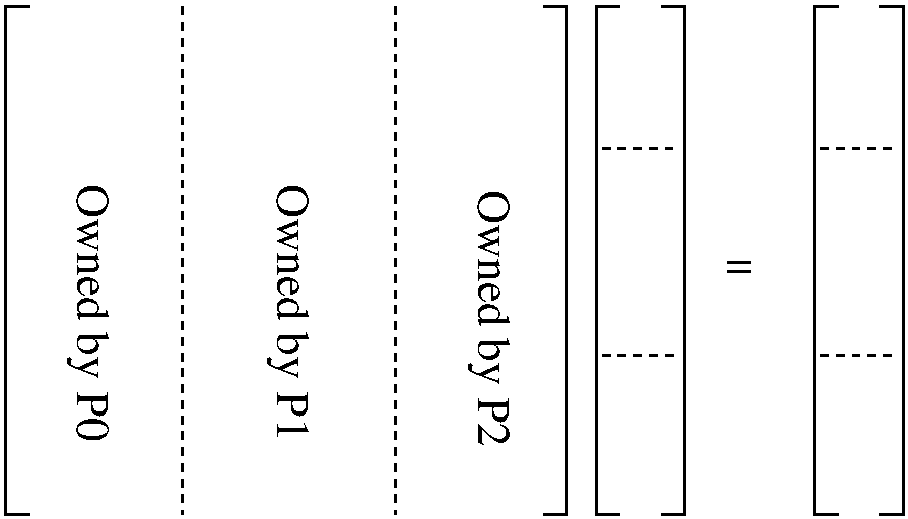
\includegraphics[width=7cm]{cols}
  \item Can be written on block form as
        \[
           \begin{bmatrix}
                \mathbf{A}_{0,0} & \mathbf{A}_{0,1} & \mathbf{A}_{0,2} \\
                \mathbf{A}_{1,0} & \mathbf{A}_{1,1} & \mathbf{A}_{1,2} \\
                \mathbf{A}_{2,0} & \mathbf{A}_{2,1} & \mathbf{A}_{2,2}
           \end{bmatrix}\begin{bmatrix}
                          \mathbf{x}_0 \\
                          \mathbf{x}_1 \\
                          \mathbf{x}_2
                        \end{bmatrix} = \begin{bmatrix}
                                          \mathbf{b}_0 \\
                                          \mathbf{b}_1 \\
                                          \mathbf{b}_2
                                        \end{bmatrix}
        \]
\end{itemize}
\end{frame}
\begin{frame}\frametitle{Matrix partitioning}
\begin{itemize}
  \item With $N$ process, we see that process $p$ can evaluate in N+1 steps;
  \begin{enumerate}
    \item Perform local MxV to obtain
        \[
          \mathbf{w} = \begin{bmatrix}
                          \mathbf{A}_{0,p}\mathbf{x}_p \\
                          \mathbf{A}_{1,p}\mathbf{x}_p \\
                          \vdots \\
                          \mathbf{A}_{N-1,p}\mathbf{x}_p
                       \end{bmatrix}
        \]
     \item Participate in $N$ reductions, e.g. to form $\mathbf{v}_0$ as
      \[
          \mathbf{v}_0 = \sum \mathbf{A}_{0,j}\mathbf{r}_j.
      \]
  \end{enumerate}
  \item Common to both these approaches is that we need to exchange the entire vector between processes.
\end{itemize}
\end{frame}
\begin{frame}\frametitle{Domain decomposition}
\begin{itemize}
  \item Very general, can be used for all kinds of grids.
    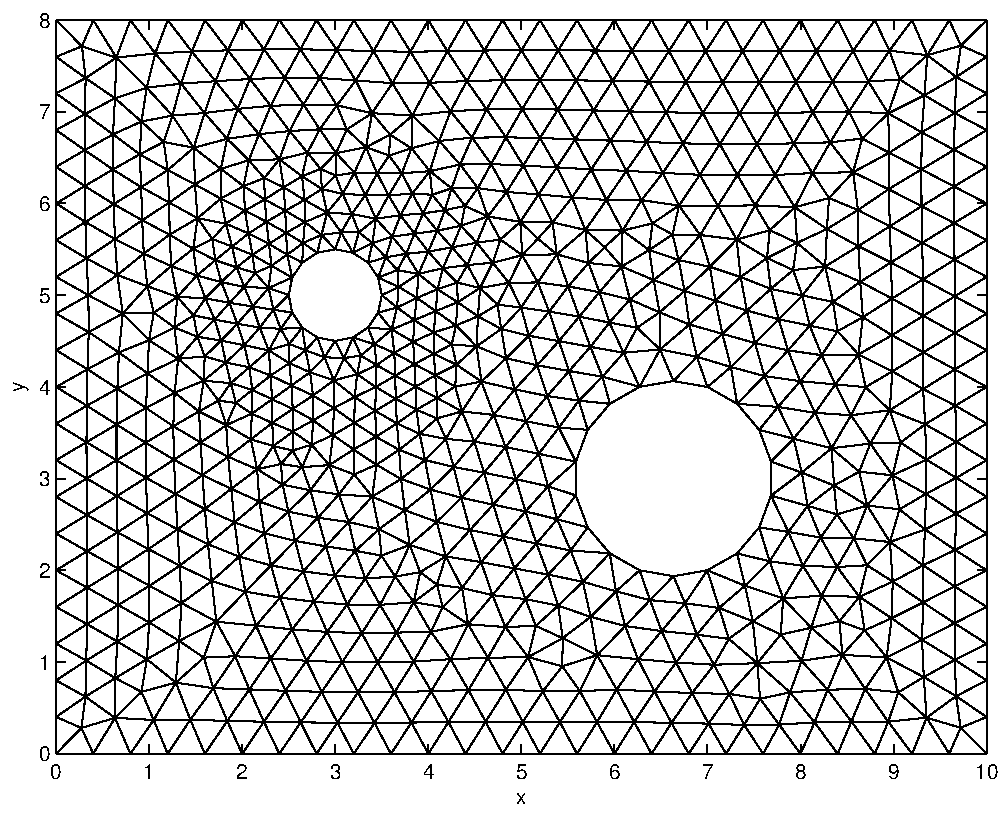
\includegraphics[width=4.5cm]{grid2D_1domain}
    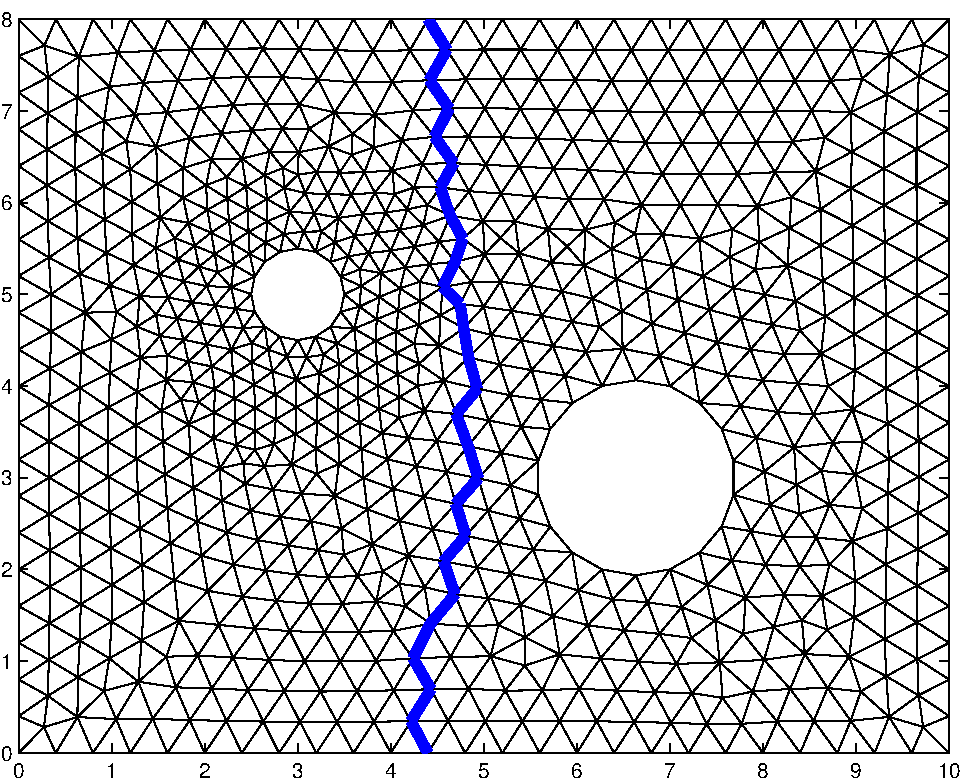
\includegraphics[width=4.5cm]{grid2D_2domains}
\end{itemize}
\end{frame}
\begin{frame}\frametitle{Gauss-Jacobi iterations - MPI parallelization}
  \begin{itemize}
    \item We partition the mesh - in 1D this is the same as splitting a vector.
      \begin{center}
        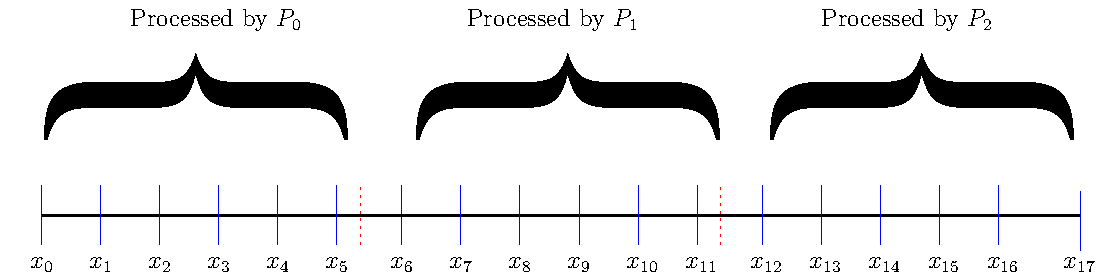
\includegraphics[width=8cm]{meshsplit}
      \end{center}
    \item On each MPI process, we use a ``redundant'' storage format - with extra elements at the start and end of the vector.
          We do this, even on processes which do not own the physical boundary.
      \begin{center}
        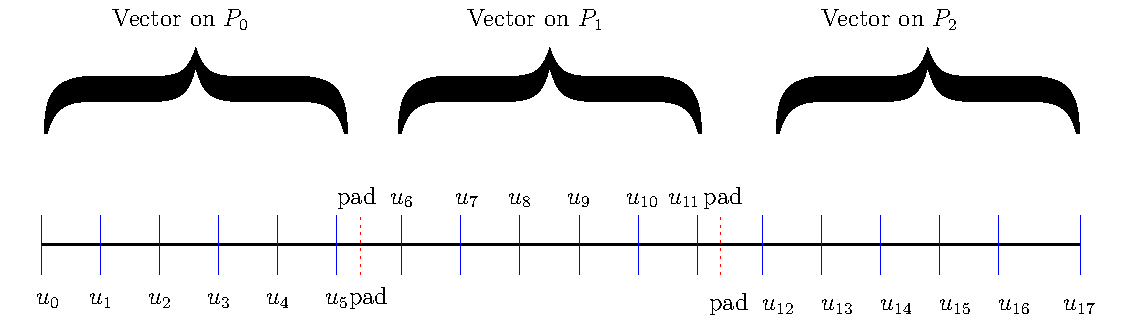
\includegraphics[width=8cm]{redundant}
      \end{center}
  \end{itemize}
\end{frame}
\begin{frame}\frametitle{Gauss-Jacobi iterations - MPI parallelization}
  \begin{itemize}
    \item We create a MPI communicator with the topology attached using
      \begin{itemize}
        \item \emph{MPI\_Dims\_create}
        \item \emph{MPI\_Cart\_create}
      \end{itemize}
    \item Each process can find its place in the topology through \emph{MPI\_Cart\_coords}.
    \item We exchange data through combined use of \emph{MPI\_Shift} and \emph{MPI\_Sendrecv}.
    \item The off-process datas are stored in the redundant data locations.
      \begin{center}
        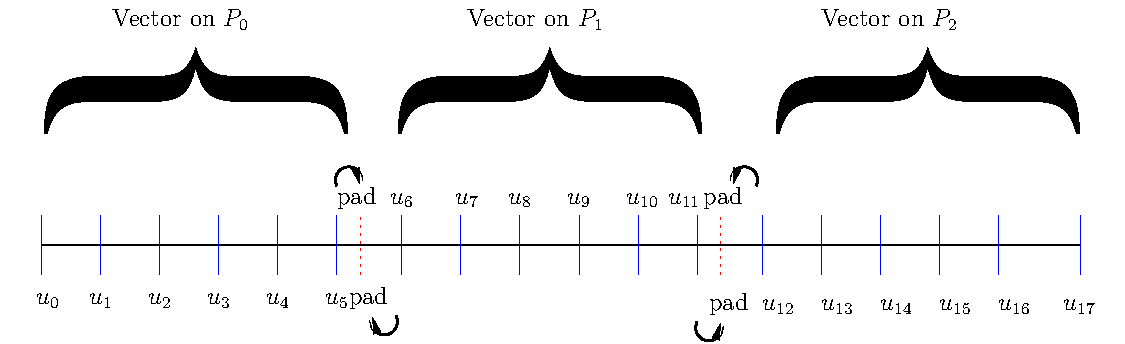
\includegraphics[width=8cm]{dataexchange}
      \end{center}
  \end{itemize}
\end{frame}
\begin{frame}\frametitle{Matrix-free Gauss-Jacobi iterations with MPI}
   \lstinputlisting[basicstyle=\tiny]{gj-mpi.c}
\end{frame}
\frame[label=mpiio14]{
  \frametitle{2D implementation - Distributed arrays}
  \begin{itemize}
    \item We store our solution in vector as a matrix for convenience. We want to partition this array.
      \begin{center}
        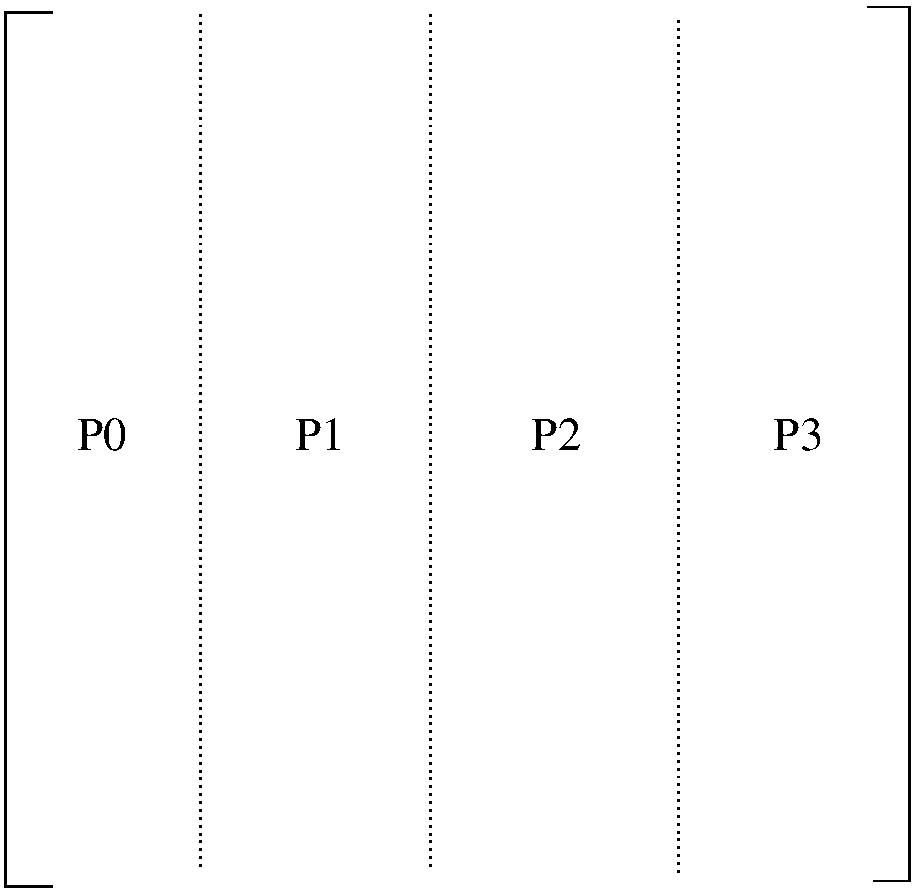
\includegraphics[width=4cm]{strip}
        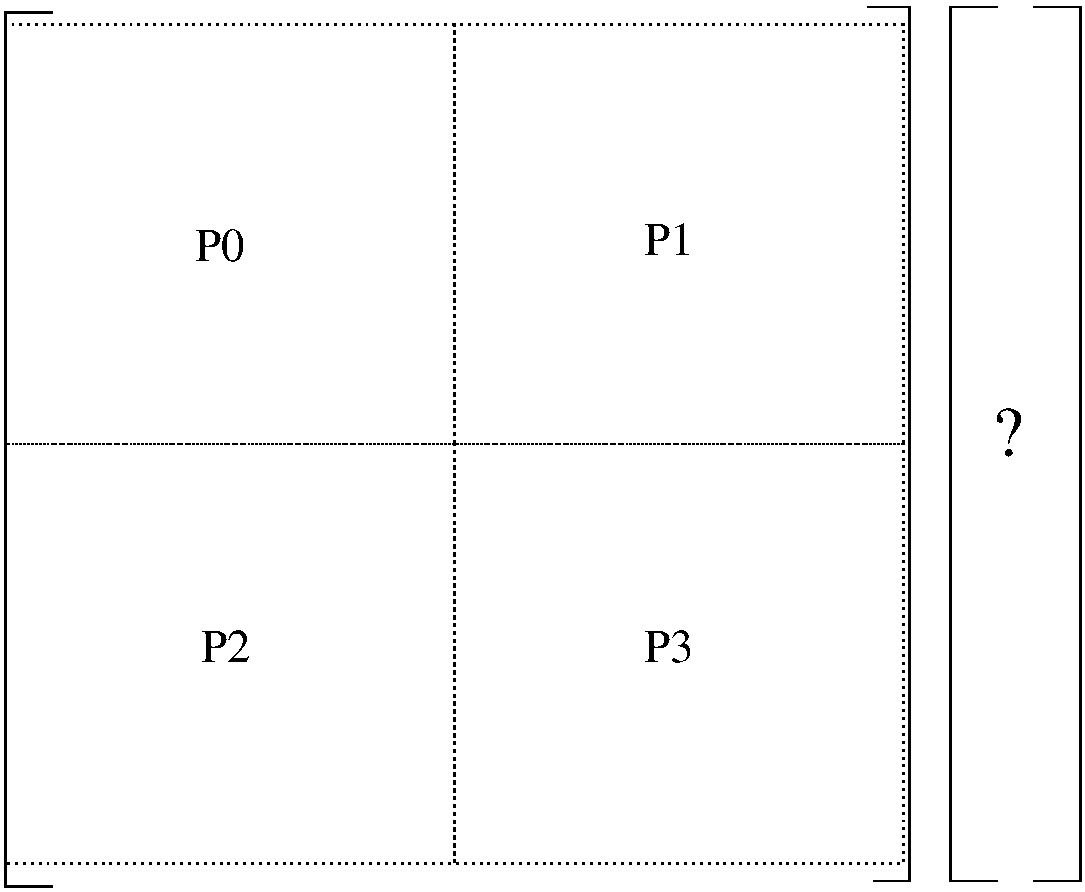
\includegraphics[width=4cm]{block}
      \end{center}
    \item The \texttt{MPI} machinery allows us to handle both of these with essentially 
      the same code.
  \end{itemize}
}
\frame[label=mpiio15]{
  \frametitle{2D implementation - distributed arrays contd.}
  \begin{itemize}
    \item \texttt{MPI} names such arrays \emph{darrays} - distributed arrays.
    \item The available functions are heavily inspired by the \texttt{High Performance Fortran}
      standard.
    \item In the following we use the term \emph{topology}, which in layman's terms means
      ``how stuff is connected''.
    \item An array partitioning consists of a topology and a mapping of processes onto this
      topology.
  \end{itemize}
}
\frame[label=mpiio16]{
  \frametitle{2D implementation - Distributed arrays contd.}
  \begin{itemize}
    \item The following figure contains the pieces of information we need to describe the
      topology and the mapping.
      \begin{center}
        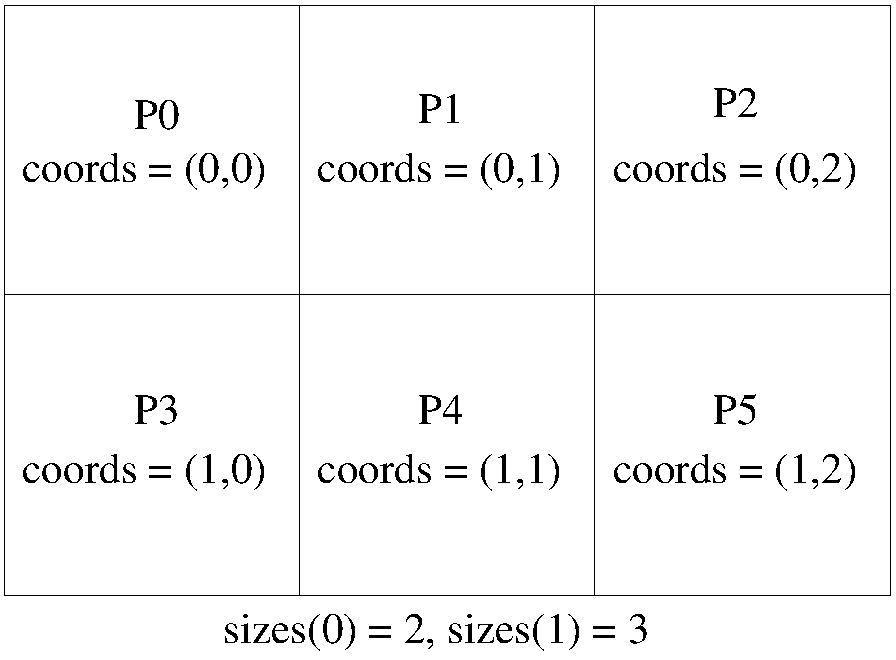
\includegraphics[width=8cm]{splitdomain}
      \end{center}
  \end{itemize}
}
\frame[label=mpiio17]{
  \frametitle{2D implementation - Distributed arrays}
  \begin{itemize}
    \item A global topology - here a Cartesian topology expressed as the number 
      of processes along each dimension (here 2 and 3, respectively).
    \item Location of a particular domain in the topology, again
      this can be expressed as an integer along each dimension.
    \item A mapping of the available processes onto the topology.
  \end{itemize}
}
\frame[label=mpiio18]{
  \frametitle{2D implementation - Distributed arrays}
  \begin{itemize}
    \item The first function we use is \emph{MPI\_Dims\_Create}. This generates
      a Cartesian partioning.
    \item Block partioning: \lstinputlisting[language=C]{dimsblock.c}
    \item Strip partioning: \lstinputlisting[language=C]{dimsstrip.c}
    \item Upon return the \emph{dims} array holds the results.
  \end{itemize}
}
\frame[label=mpiio19]{
  \frametitle{2D implementation - Distributed arrays}
  \begin{itemize}
    \item In order to be able to generate the mapping of processes onto
      the topology, we need to define a communicator which has the
      topology attached.
      \lstinputlisting[language=C]{comm.c}
    \item Upon return the \emph{comm} variable holds the new communicator.
  \end{itemize}
}
\frame[label=mpiio20]{
  \frametitle{2D implementation - Distributed arrays}
  \begin{itemize}
    \item The individual process can now query where they are placed in the
      topology using the function
      \lstinputlisting[language=C]{coord.c}
    \item Upon return from the function, the \emph{coords} array holds the coordinates.
      For instance, it would hold 1 and 2 when called on process 5.
  \end{itemize}
}
\begin{frame}\frametitle{Another class of iterative methods: Krylov methods}
  \begin{itemize}
    \item Another very important classes of iterative methods are the Krylov subspace methods.
    \item Observation:
      \[
        \ub{x} = \sum_{j=0}^{N-1} v_j\ub{A}^j \ub{b}
      \]
      for any vector $\ub{b}$, that is $\text{span}\left\{\ub{A}^j\ub{b}\right\}_{j=0}^{N-1}$ form a basis for
      the column space of $\ub{A}$. We call this space the Krylov subspace of $\ub{A}$. Here $v_j$ is a set of coefficients.
    \item Idea of Krylov subspace methods; make an initial guess, then
      improve this by successively eliminating contributions to the
      residual along each Krylov vectors.
  \end{itemize}
\end{frame}

\begin{frame}\frametitle{Another class of iterative methods: Krylov methods}
  \begin{itemize}
    \item Many different Krylov methods, suitable for different types of
        linear systems (in the sense of symmetries, definiteness etc).
    \item The two maybe most important ones;
      \begin{itemize}
        \item GMRES - the generalized minimum residual method.
              This is the ``hammer'' in the sense that it handles non-symmetric
              and non-definite problems.
        \item CG - the conjugate gradient method.
              This works for symmetric, positive definite systems.
      \end{itemize}
    \item In the following: we only consider CG.
  \end{itemize}
\end{frame}

\begin{frame}\frametitle{The conjugate gradient algorithm}
\begin{center}
  \boxed{
    \begin{minipage}{8cm}
      \begin{align*}
        \text{Set } \underline{u}^0 &= \underline{0}, \quad \underline{r}^0 = \underline{f}  \nonumber \\
        \text{For } m&=1,2,\ldots \nonumber \\
        \beta_m &= \frac{(\underline{r}^{m-1})^T \underline{r}^{m-1}}{(\underline{r}^{m-2})^T \underline{r}^{m-2}} \qquad \quad (\beta_1 \equiv 0) \nonumber \\
        \underline{p}^m &= \underline{r}^{m-1} + \beta_m \underline{p}^{m-1} \qquad (\underline{p}^1 \equiv \underline{r}^0) \\
        \alpha_m &= \frac{(\underline{r}^{m-1})^T \underline{r}^{m-1}}{(\underline{p}^{m})^T \underline{A} \underline{p}^m} \nonumber \\
        \underline{u}^m &= \underline{u}^{m-1} + \alpha_m \underline{p}^m \nonumber \\
        \underline{r}^m &= \underline{r}^{m-1} - \alpha_m \underline{A} \underline{p}^m \nonumber \\
        \text{end}\quad&
      \end{align*}
    \end{minipage}
  } 
\end{center}
\end{frame}

\begin{frame}\frametitle{The conjugate gradient algorithm}
  \begin{itemize}
    \item These are hybrid methods - eliminate along all Krylov vectors
        and we get the exact solution (if done with exact arithmetics).
    \item We use this as a way to obtain an approximative solution  
      by introducing a stopping criterion.
    \item Typical stopping criterion:
      \[
        \|r\| < tol
      \]
      for some tolerance $tol$.
  \end{itemize}
\end{frame}

\begin{frame}\frametitle{The conjugate gradient algorithm}
  \begin{itemize}
    \item An implementation may look like:
      \lstinputlisting[basicstyle=\tiny]{cg.c}
  \end{itemize}
\end{frame}
\end{document}
